%%%%%%%%%%%%%%%%%%%%%%%%%%%%%%%%%%%%%%%%%
% University/School Laboratory Report
% LaTeX Template
% Version 3.1 (25/3/14)
%
% This template has been downloaded from:
% http://www.LaTeXTemplates.com
%
% Original author:
% Linux and Unix Users Group at Virginia Tech Wiki 
% (https://vtluug.org/wiki/Example_LaTeX_chem_lab_report)
%
% License:
% CC BY-NC-SA 3.0 (http://creativecommons.org/licenses/by-nc-sa/3.0/)
%
%%%%%%%%%%%%%%%%%%%%%%%%%%%%%%%%%%%%%%%%%

%----------------------------------------------------------------------------------------
%	PACKAGES AND DOCUMENT CONFIGURATIONS
%----------------------------------------------------------------------------------------

\documentclass{article}

%\usepackage[version=3]{mhchem} % Package for chemical equation typesetting
%\usepackage{siunitx} % Provides the \SI{}{} and \si{} command for typesetting SI units
\usepackage{graphicx} % Required for the inclusion of images
\usepackage[section]{placeins}
\usepackage{booktabs} % For prettier tables
\usepackage{float} % To control positions of e.g. tables or figures
\usepackage[colorlinks]{hyperref} % To color blocks of text 
\usepackage[dvipsnames]{xcolor} % More color options (see Wikibooks)  
\usepackage{changepage}
%\usepackage[dvipdfmx]{graphicx}
%\usepackage{bmpsize} % Added at some point but now (June-16) it seems to do nothing
%\usepackage{natbib} % Required to change bibliography style to APA
%\usepackage{amsmath} % Required for some math elements 

\graphicspath{{/home/totta/Ef\_RNAseq/figures\_and\_manuscript/}}
\setlength\parindent{0pt} % Removes all indentation from paragraphs

\renewcommand{\labelenumi}{\alph{enumi}.} % Make numbering in the enumerate environment by letter rather than number (e.g. section 6)

%\usepackage{times} % Uncomment to use the Times New Roman font
%----------------------------------------------------------------------------------------
%	DOCUMENT INFORMATION
%----------------------------------------------------------------------------------------

\title{Data summary and analysis procedure: dual RNA-seq of \textit{Eimeria falciformis} infected \textit{Mus musculus}} % Title

\author{Totta \textsc{Kasemo}, Simone \textsc{Spork},\\ Christoph \textsc{Dietrich}, Richard \textsc{Lucius}, Emanuel \textsc{Heitlinger}} % Author name

\date{\today} % Date for the report

\begin{document}

\maketitle % Insert the title, author and date

\begin{center}
\begin{tabular}{l r}
%Date Performed: & January 1, 2012 \\ % Date the experiment was performed
%Partners: & James Smith \\ % Partner names
%& Mary Smith \\
%Instructor: & Professor Smith % Instructor/supervisor
\end{tabular}
\end{center}

% If you wish to include an abstract, uncomment the lines below
% \begin{abstract}
% Abstract text
% \end{abstract}

%----------------------------------------------------------------------------------------
%	SECTION 1
%----------------------------------------------------------------------------------------

\section{Overview}
This document contains data summaries and parts of analysis from the dual RNA-seq experiments of 
 \textit{Eimeria falciformis} infected mice carried our by Simone Spork. Basic read-outs
 such as number of transcripts detected in each sample from mouse and parasite are summarized, as
 well as compilations of the outcome of statistical tests for differential mRNA abundance from
 comparisons of different experimental groups. Mouse data was compared (correlated) with previously
 published (schmid12) microarray data from \textit{E. falciformis} infected mice.
 Hierarchical clustering illustrated by heatmaps is shown for different comparisons.\\
 The largest mRNA abundance differences on the parasite side are seen in comparisons between different
 time points post infection. Mouse strain, including Rag1-/- (adaptive immunity compromised mice) and 
 mouse immune status due to previous parasite exposure (second/challenge infection) seems to have less effects
 on mRNA abundance profiles in the parasite.
%\begin{center}\ce{}\end{center}

%----------------------------------------------------------------------------------------
%	SECTION  
%----------------------------------------------------------------------------------------

%%%%%%%%%%%%%%%%%%%%%%%%%%%%%%%%%
%	METHODS
%%%%%%%%%%%%%%%%%%%%%%%%%%%%%%%%%
\section{Methods}
\subsection{Mice and infection procedure}
Three strains of mice were used in our experiments: NMRI (Charles River Laboratories, Sulzfeld,
Germany), C57BL/6 (), and Rag1-/- on C57BL/6 background (gift from Susanne Hartmann, FU?). 
Animal procedures were performed according to the German Animal Protection Laws as 
directed and approved by the overseeing authority Landesamt fuer Gesundheit und Soziales 
(Berlin, Germany). Animals where infected as described by Schmid et al., (Schmid12), but
tapwater was used instead of PBS for administration of oocysts. Briefly, NMRI mice were infected 
two times, which will be referred to as first and second infection. For the first infection, 
150 sporulated oocysts were administered in 100 $μ$L by oral gavage. During the first infection
of 60 mice, all animals were weighed every day. On day zero, before infection, as well as on day three,
five and seven days post infection, dpi, caeca from 3-4 sacrificed mice per time point were 
collected. Epithelial cells were isolated as described in Schmid et al.(schmid12). For challenge 
infection, mice recovered for four weeks before second infection. 
Recovery was monitored by weighing and visual inspection of fur. For the second infection, 
1500 sporulated oocysts were applied by oral gavage. Three mice were used as non-second infection control, 
referred to as day 0, second infection.

\subsection{Oocyst purification for infection and sequencing}
Sporulated oocysts were purified by flotation from feces stored in potassium dichromate and 
administered orally in 100 uL tapwater. One \textit{E. falciformis} isolate, 
\textit{E. falciformis} Bayer Haberkorn 1970, was used for all infections and parasite 
samples. The strain is maintained through passage in NMRI mice in our facilities as described 
elsewhere (schmid12).

\subsection{Sporozoite isolation}
Sporozoites were isolated from sporocysts by excystment. For this, sporocysts were incubated at 
37$°$C in DMEM containing 0.04\% tauroglycocholate (MP Biomedicals) and 0.25\% trypsin (Applichem) 
for 30 min. Sporozoites were purified by the method of Schmatz et al (schmatz--).

\subsection{RNA extraction}
Total RNA was isolated from infected epithelial cells, sporozoites and sporulated oocysts 
using Trizol according to the manufacturer’s protocol (Invitrogen). High quality  \emph{what is the meaning of 'high quality' here?}
RNA was used to produce an mRNA library using the Illumina’s TruSeq RNA Sample Preparation guide.
\emph{stolen from genome paper}
Sporozoites were stored in 1 mL Trizol until RNA-isolation. 
Total RNA was isolated using the PureLink RNA Mini Kit (Invitrogen).

\subsection{Sequence quality assessment and alignment}
Fastq\_quality\_filter was applied to Illumina Hiseq 2000 sequenced samples. 
Since this is not easily applicable to pair-end sequencing data, a low threshold was 
used on the hiseq data. A phred score of 10 was used, i.e., the probability of false base 
calling is one in ten. We further set q = 60, i.e., nine out of ten bases
or more is required to be correct in at least 
60\% of the bases in each read for the read sequence to be kept for further analysis.
This resulted in.......

\subsubsection{Alignment and reference genomes}
We used the published \textit{Mus musculus} mm10 assembly (Genome Reference Consortium Mouse 
Build 38, GCA\_000001635.2) as reference genome including annotations for mouse data. The
\textit{E. falciformis} genome (Heitlinger14) was downloaded from ToxoDB (Gajria07). For the
alignment, the mouse and parasite genome files were merged into a dual reference genome, and 
files including mRNA sequences from both species were aligned against the dual reference genome
using TopHat2 (version 2.0.14, Trapnell09)/ Bowtie2 (version 1.1.2, Langmead12). Single-end and 
pair-end sequence samples were aligned separately with library type 'fr-unstranded' specified 
for pair-end samples. Import into R was enabled by the R package Ballgown, which requires bam 
files to be processed by Tablemaker (Frazee15). Tablemaker in turn makes use of Cufflinks 
(version 2.1.1, Trapnell10).



%----------------------------------------------------------------------------------------
%	SECTION  
%----------------------------------------------------------------------------------------


\section{Table of reads per sample}
% latex table generated in R 3.2.2 by xtable 1.8-2 package
% Wed Mar  2 14:36:30 2016
\setlength{\tabcolsep}{10pt}
\begin{table}[H]
\centering 
	\caption{Reads per sample listed.}
\begin{tabular}{*5l}    \toprule
Samples  & Mouse 	& \textit{E. falciformis}  & Percentage			& \#\textit{E.falciformis} \\
	& trancripts	& transcripts   	 & \textit{E. falciformis}	& genes \\ \midrule
NMRI\_oocysts\_rep1 & 11676.000 & 108477484.000 & 99.989 & 5734.000 \\ 
NMRI\_oocysts\_rep2 & 19024.000 & 126543533.000 & 99.985 & 5774.000 \\ 
NMRI\_sporozoites\_rep1 & 13800.000 & 92259539.000 & 99.985 & 5808.000 \\ 
NMRI\_sporozoites\_rep2 & 8702.000 & 21508353.000 & 99.960 & 5564.000 \\ 
NMRI\_1stInf\_7dpi\_rep1 & 12532238.000 & 79648900.000 & 86.405 & 5894.000 \\ 
NMRI\_1stInf\_7dpi\_rep2 & 94310278.000 & 154343046.000 & 62.072 & 5897.000 \\ 
NMRI\_1stInf\_5dpi\_rep3 & 334671421.000 & 54022504.000 & 13.899 & 5794.000 \\ 
NMRI\_2ndInf\_7dpi\_rep1 & 97221189.000 & 9927803.000 & 9.265 & 5865.000 \\ 
NMRI\_1stInf\_5dpi\_rep1 & 204647381.000 & 18549727.000 & 8.311 & 5739.000 \\ 
C57BL6\_1stInf\_5dpi\_rep2 & 32887009.000 & 250954.000 & 0.757 & 3946.000 \\ 
	{\color{Gray}NMRI\_2ndInf\_5dpi\_rep1} & {\color{Gray} 589643389.000} & {\color{Gray}3752923.000} & {\color{Gray} 0.632} &  {\color{Gray}5602.000} \\ 
NMRI\_1stInf\_5dpi\_rep2 & 316721928.000 & 1609009.000 & 0.505 & 5439.000 \\ 
C57BL6\_2ndInf\_5dpi\_rep1 & 62053975.000 & 311900.000 & 0.500 & 4610.000 \\ 
	{\color{Gray}NMRI\_1stInf\_3dpi\_rep1} & {\color{Gray}209723287.000} &  {\color{Gray}815820.000} &  {\color{Gray}0.388} &  {\color{Gray}5466.000} \\ 
C57BL6\_1stInf\_5dpi\_rep1 & 65523435.000 & 217606.000 & 0.331 & 4259.000 \\ 
Rag\_2ndInf\_5dpi\_rep1 & 85288323.000 & 224273.000 & 0.262 & 4251.000 \\ 
Rag\_1stInf\_5dpi\_rep2 & 57192380.000 & 113673.000 & 0.198 & 2969.000 \\ 
NMRI\_1stInf\_3dpi\_rep2 & 515516785.000 & 903330.000 & 0.175 & 5101.000 \\ 
Rag\_1stInf\_5dpi\_rep1 & 71173382.000 & 73445.000 & 0.103 & 2748.000 \\ 
NMRI\_2ndInf\_7dpi\_rep2 & 122999109.000 & 46700.000 & 0.038 & 2174.000 \\ 
NMRI\_2ndInf\_3dpi\_rep2 & 106446839.000 & 34699.000 & 0.033 & 1901.000 \\ 
	 {\color{Gray}NMRI\_1stInf\_0dpi\_rep1} &  {\color{Gray}229165002.000} & {\color{Gray} 31459.000} &  {\color{Gray}0.014} & {\color{Gray} 1380.000} \\ 
NMRI\_2ndInf\_5dpi\_rep2 & 113957667.000 & 12692.000 & 0.011 & 539.000 \\ 
NMRI\_2ndInf\_3dpi\_rep1 & 91352242.000 & 5355.000 & 0.006 & 121.000 \\ 
NMRI\_2ndInf\_0dpi\_rep2 & 90681785.000 & 3738.000 & 0.004 & 62.000 \\ 
Rag\_0dpi\_rep1 & 43414004.000 & 474.000 & 0.001 & 2.000 \\ 
C57BL6\_0dpi\_rep1 & 53877840.000 & 491.000 & 0.001 & 2.000 \\ 
C57BL6\_0dpi\_rep2 & 76753491.000 & 657.000 & 0.001 & 2.000 \\ 
Rag\_0dpi\_rep2 & 80702547.000 & 730.000 & 0.001 & 3.000 \\ 
NMRI\_2ndInf\_0dpi\_rep1 & 285032128.000 & 326.000 & 0.000 & 2.000 \\ 
\bottomrule
\hline
\end{tabular}
\end{table}

Samples are listed from highest to lowest percentace of \textit{E. falciformis} transcripts per total number of transcripts (mouse plus \textit{E. falciformis}). Corresponding number of \textit{E. falciformis} genes are shown. Gray indicates that samples are excluded from analysis (see Methods for details)


%%%%%%%%%%%%%%%%%%%%%%%%%%%%%%%%%%%%%%%%%%%%%%%%%%%%%%%%%%%%%%%%%%%%%%%%%%
%% 	OVERVIEW READS PER SAMPLE, LAYOT AS EXPERIMENTAL OVERVIEW
%%%%%%%%%%%%%%%%%%%%%%%%%%%%%%%%%%%%%%%%%%%%%%%%%%%%%%%%%%%%%%%%%%%%%%%%%%

%%%%%%%% in main MS %%%%%%%%%%%%%%%%%%

%\section{Experimental overview}
%	\setlength{\tabcolsep}{14pt}
%	\begin{table}[H]
%	\begin{center}
%	\caption{Experimental overview.}
%\begin{tabular}{*4l}    \toprule
%\textit{Day, 1st infection}  	& NMRI  & C57BL/6  & Rag1-/- \\ \midrule
%	0 (control)    & $10^4$ / $10^8$  & $10^2$ / $10^8$  & $10^2$ / $10^7$  \\ %rep1/rep2, NA=no replicate
%3  		& $10^5$ / $10^8$ & NA  & NA \\ 
%5  		& $10^7$ / $10^8$ & $10^5$ / $10^7$  & $10^5$ / $10^7$ \\
%7  		& $10^8$ / $10^7$ & NA  & NA \\ 
%Oocysts 	& $10^8$ / NA & NA  & NA \\ 
%Sporozoites 	& $10^7$ / NA & NA  & NA \\ \midrule
%
%\textit{Day, 2nd infection}  	\\ \midrule
%0 (control)     & $10^3$ / $10^8$  &  NA  & NA  \\ %rep1/rep2, NA=no replicate
%3  		& $10^4$ / $10^8$ & NA  & NA \\ 
%5  		& $10^4$ / $10^8$ & $10^5$ / $10^7$  & $10^5$ / $10^7$ \\
%7  		& $10^6$ / $10^8$ & NA  & NA \\ 
%	
%	
%	\bottomrule
% \hline
%\end{tabular}
%\end{center}
%\end{table}
%
%Replicate average of transcripts as order of magnitude for \textit{E. falciformis}/mouse. 
%Columns represent mouse strains used in infection experiments. Rows represent timepoints post 
%infection plus oocyst and sporozoite samples. The upper part of the table shows data for first 
%infection, and oocyst and sporozoite data. The lower part shows data for challenge infection. 
%Averages were calculated after sample exclusions (see Methods). For exact values, see Table 1.

%%%%%%%%%%%%%%%%%%%%%%%%%%%%%%%%%%%%%%%%%%%%%%%%%%%%%%%%%%%%%%%%%%%%%%%%%%
%% 	MICROARRAY COMPARISON
%%%%%%%%%%%%%%%%%%%%%%%%%%%%%%%%%%%%%%%%%%%%%%%%%%%%%%%%%%%%%%%%%%%%%%%%%%
\section{Transcript coverage distribution and sample exclusions}
\subsection{Mouse transcript distributions}
\begin{figure}[H]
\centering
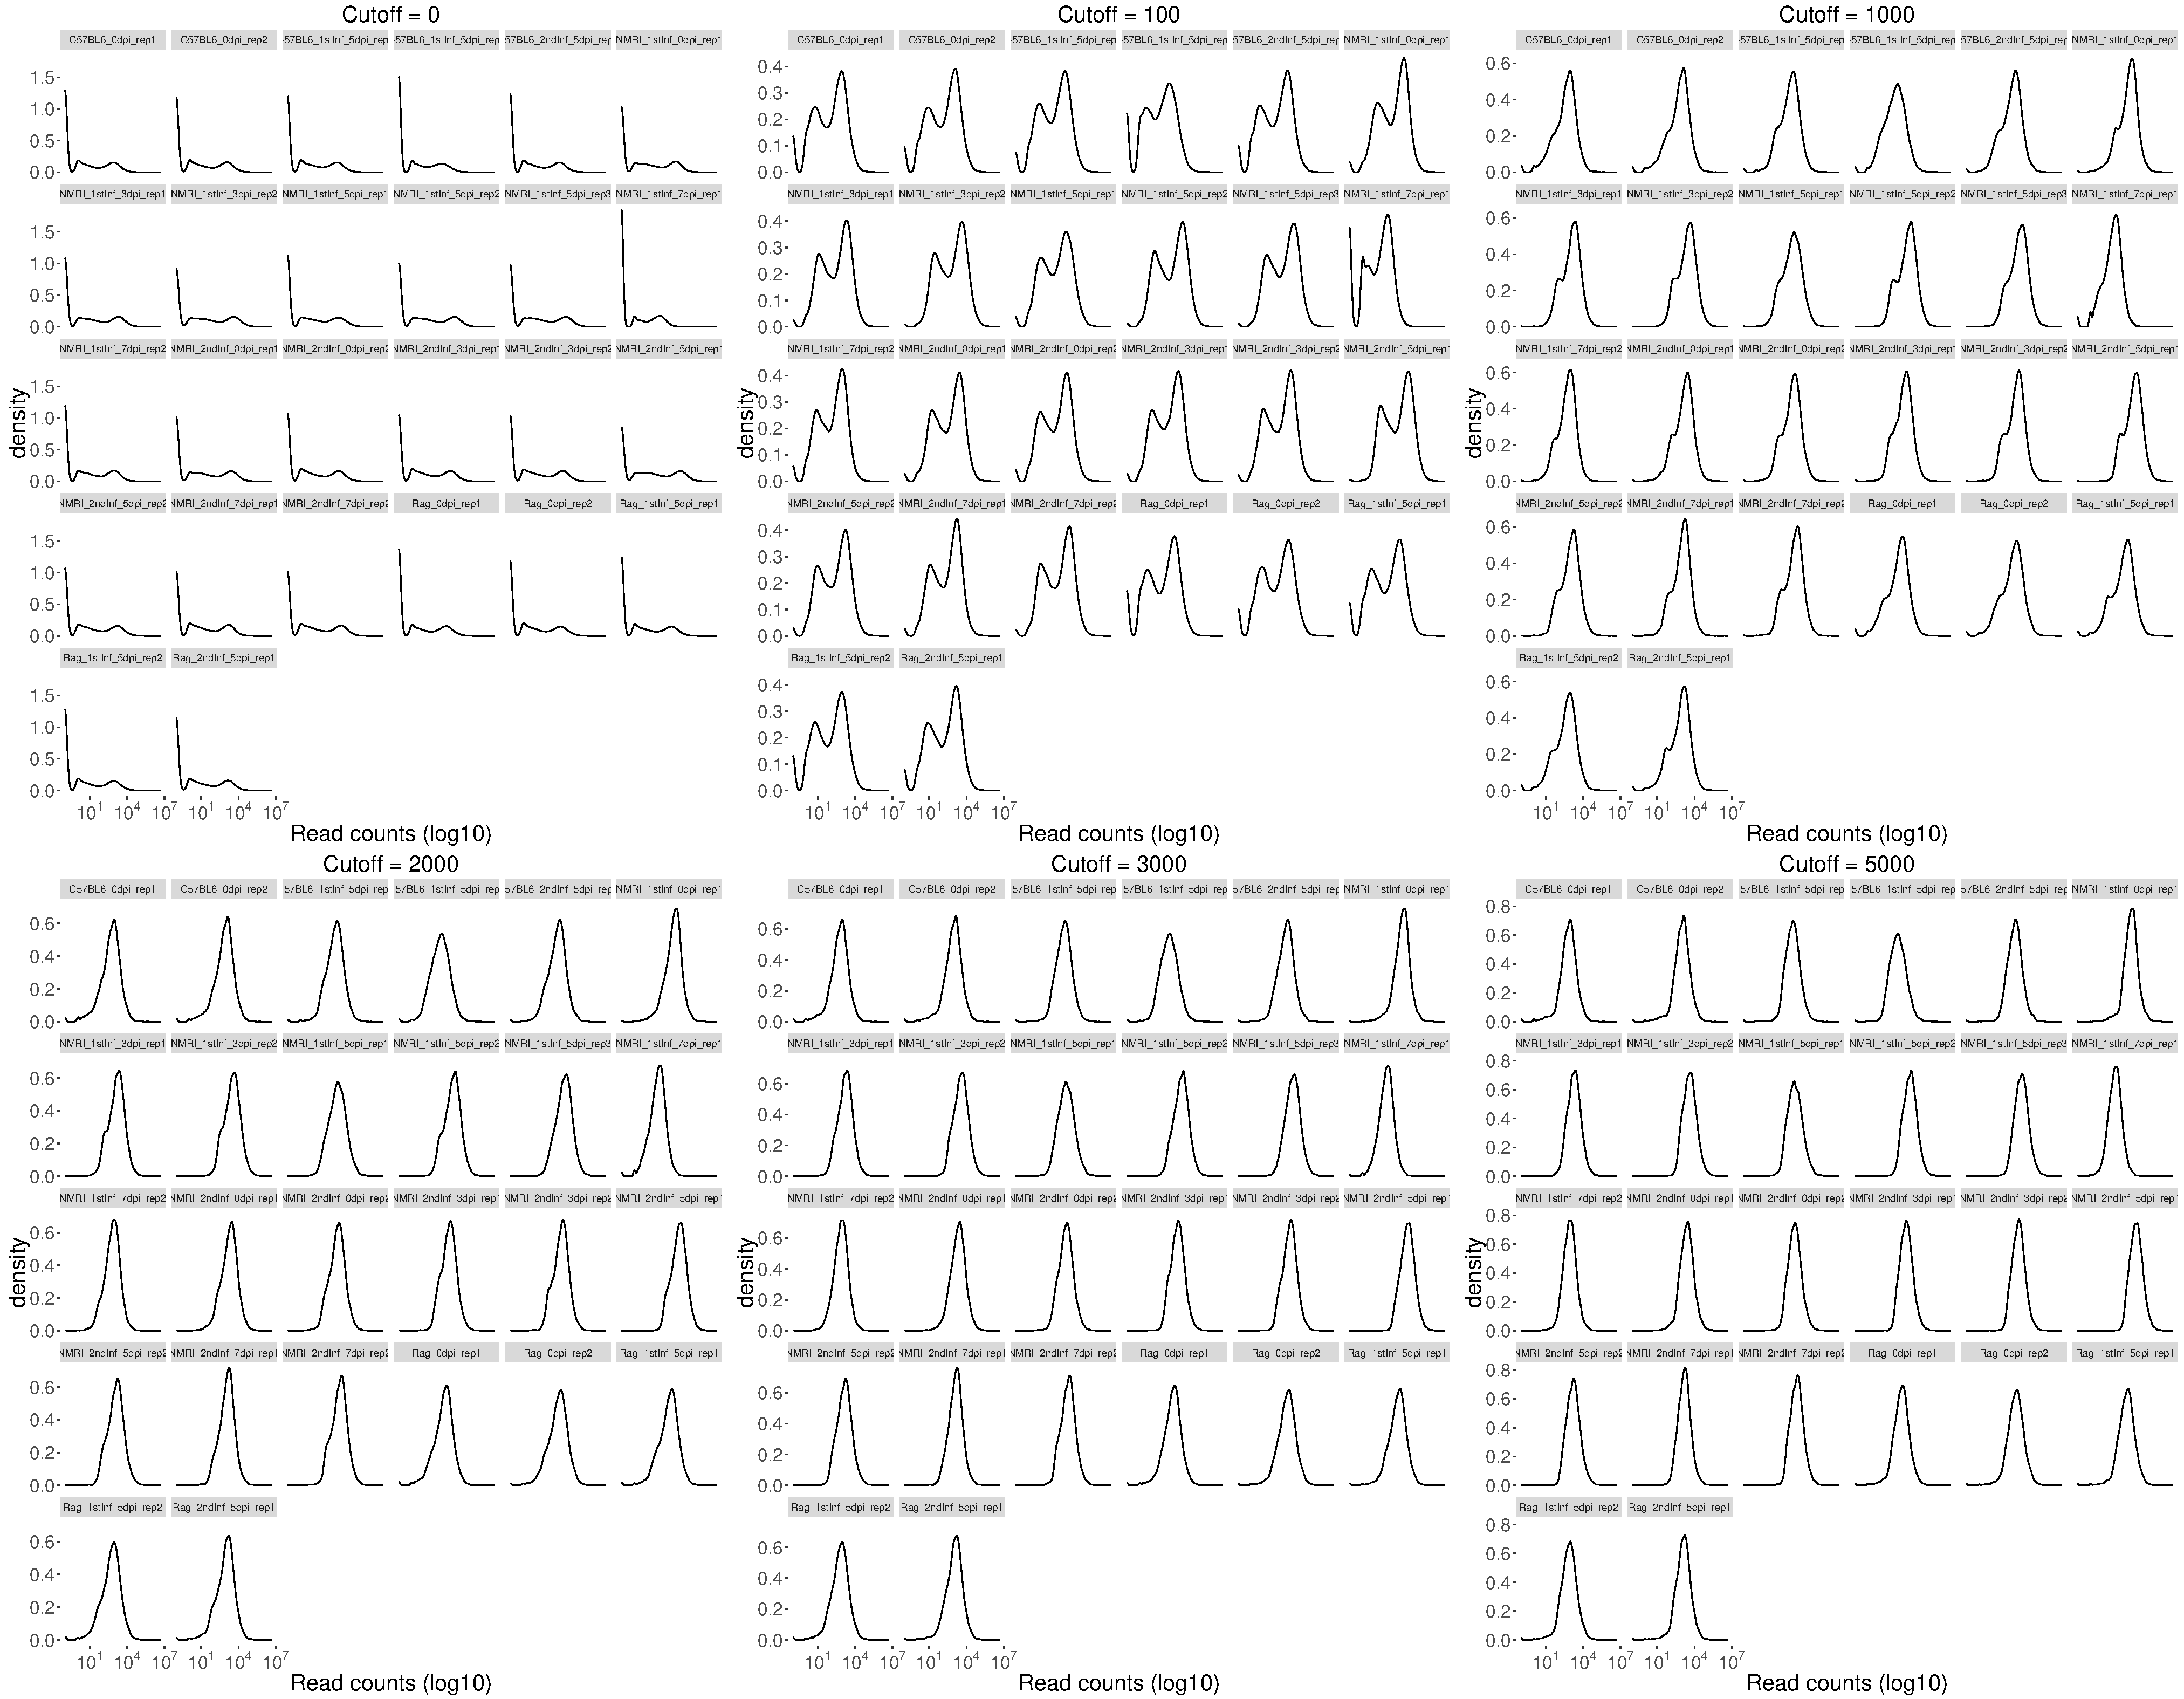
\includegraphics[width=\textwidth]{distributionsMm.pdf}
	\caption{Transcript coverage distribution (density) for mouse samples. 
 Without cutoff for a minimum read coverage over all samples, all samples display a bimodal distribution trend and an additional peak at zero by visual inspection. In our analyses, a cutoff of 3000 was applied.With this cutoff we can assume a negative binomial coverage distribution as required in the analysis pipline. Non-normalised read counts were used. For this visualization 0.1 was added to all read counts to allow to plot absent transcripts (zero reads) on a log-scale.}
%\end{center}
\end{figure}

\clearpage
\subsection{\textit{E. falciformis} transcript distributions}
\begin{figure}[H]
\begin{center}
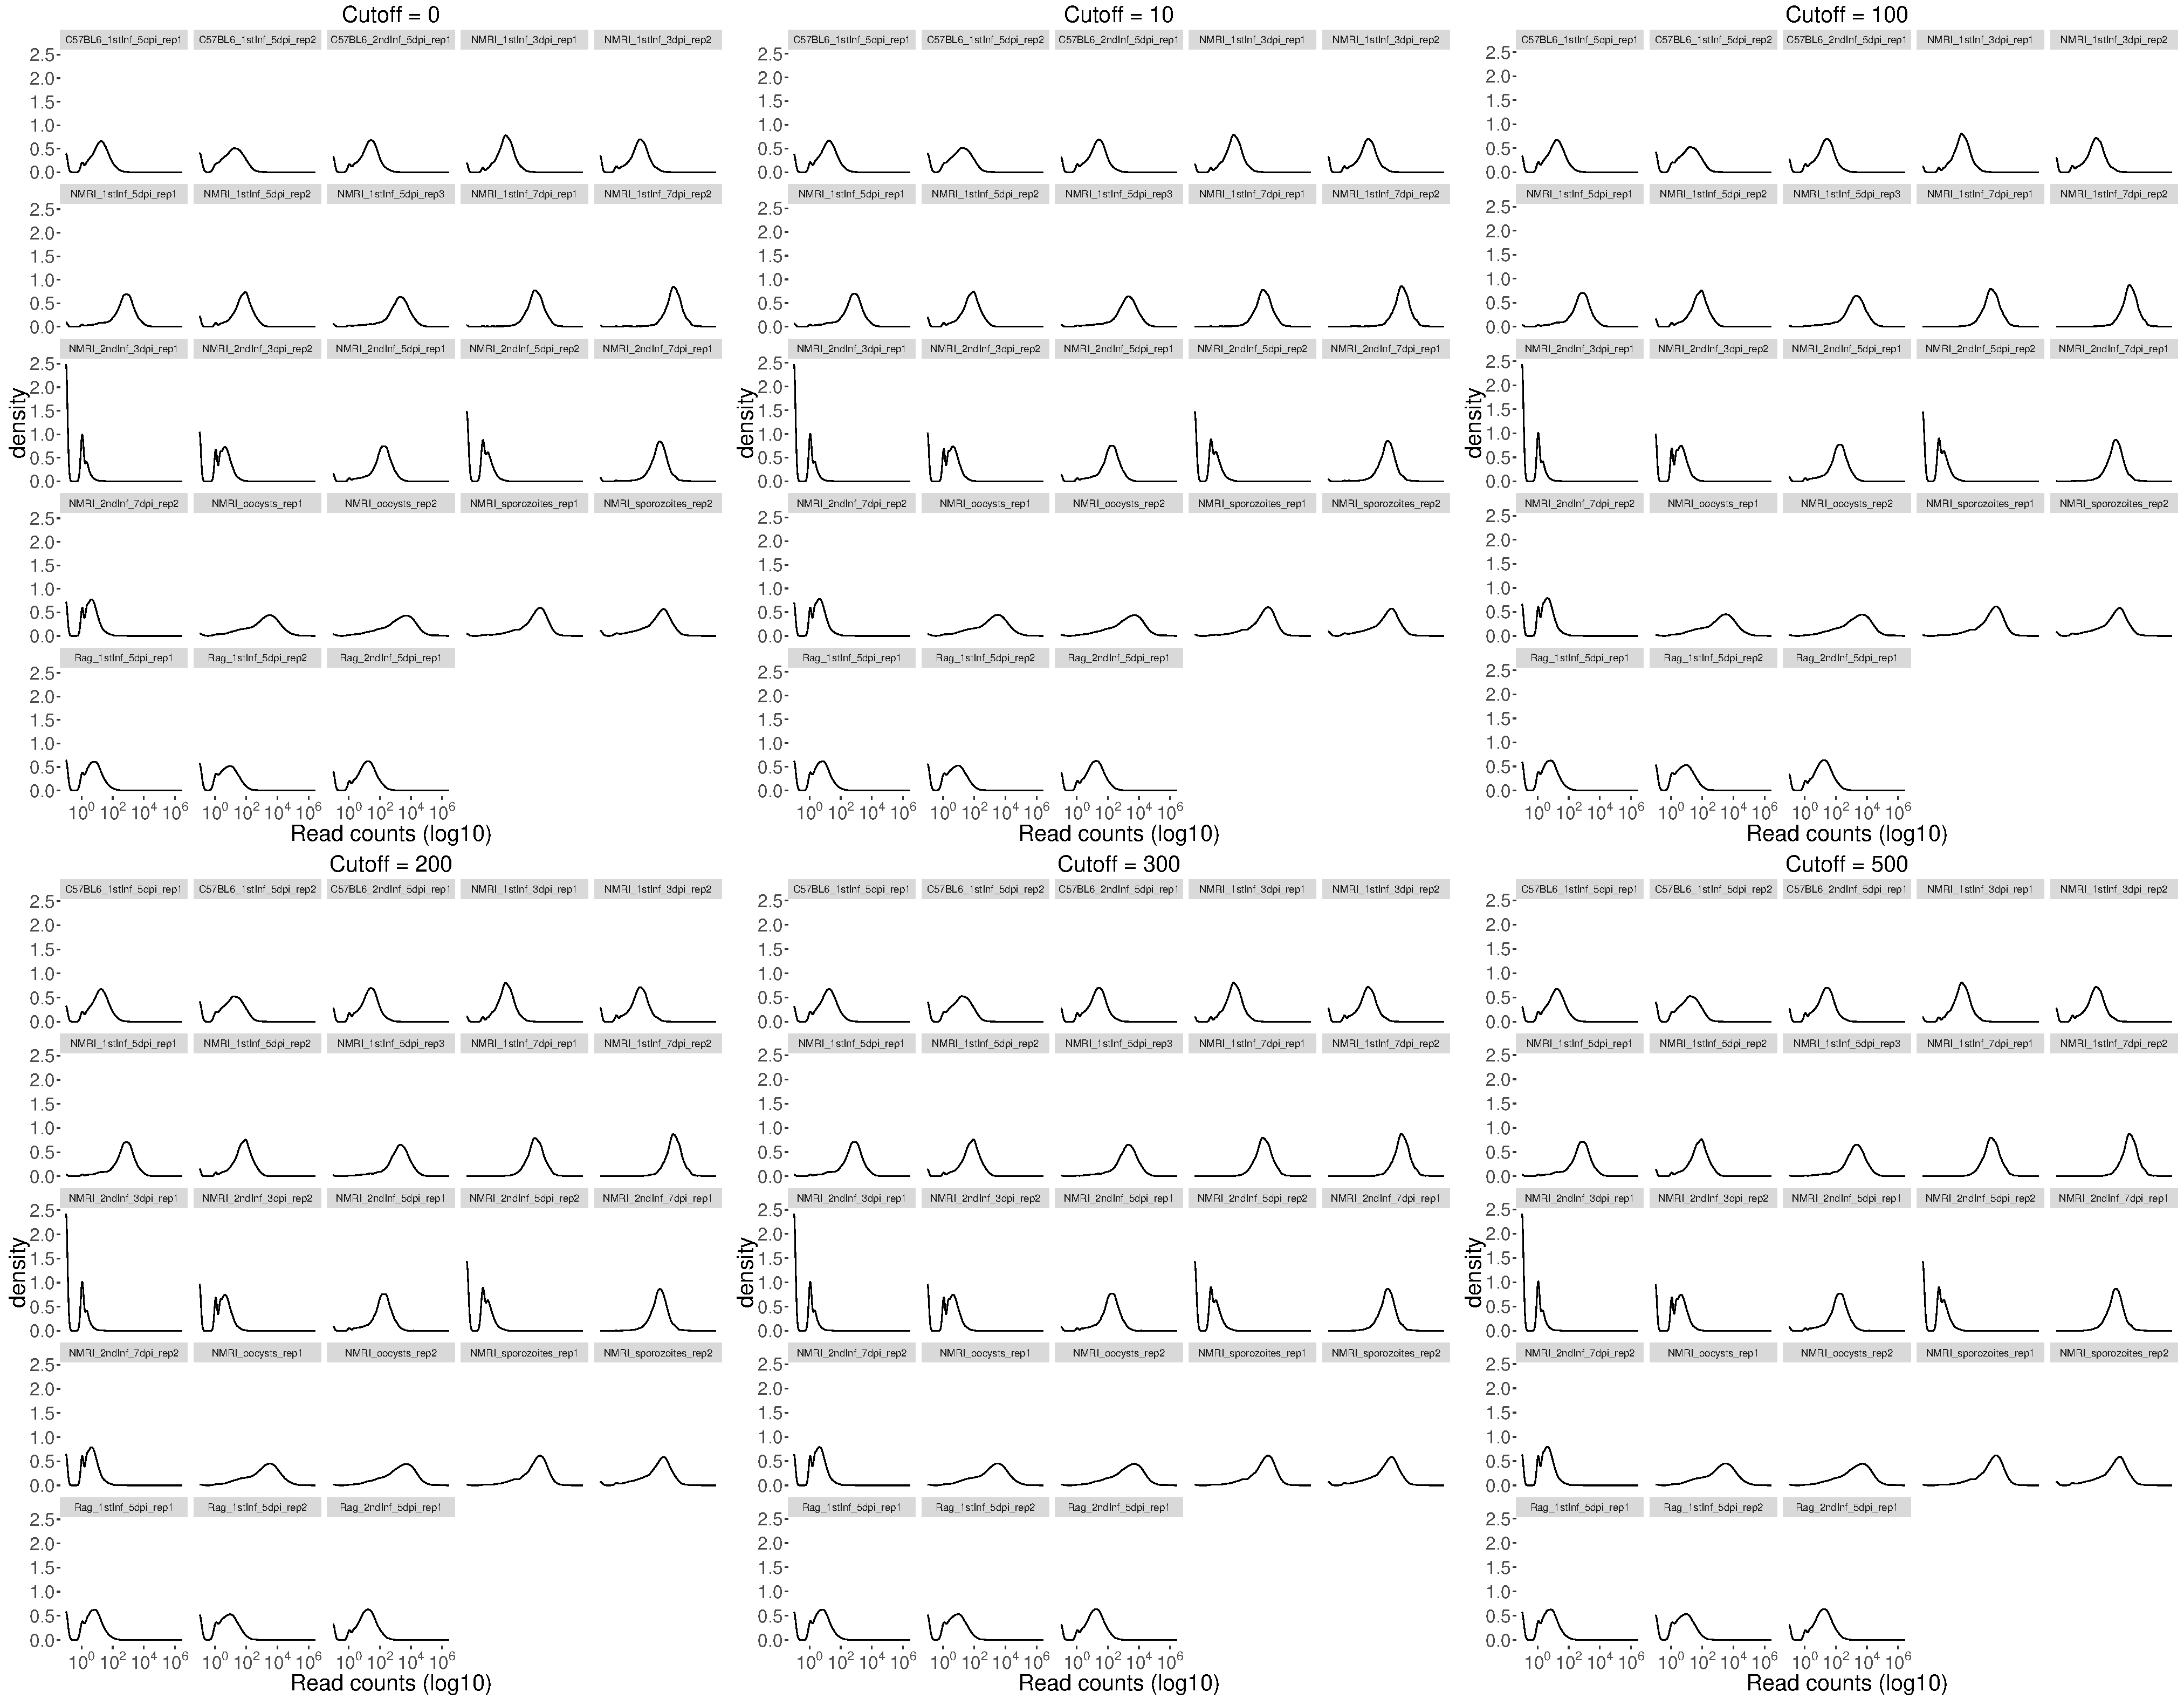
\includegraphics[width=\textwidth]{distributionsEf.pdf}
\caption{Transcript coverage density distribution density for \textit{E. falciformis} samples. Without cutoff for a minimum read coverage over all samples, most samples are in agreement with the assumed negative binomial distribution. However, two samples contradict this assumption and a cutoff was applied to evaluate whether peaks in these samples can be removed by excluding transcripts with very low coverage. The cutoff does not have a large effect on distributions and therefore two samples were removed from further 
analysis: NMRI\_1st\_3dpi\_rep1 and NMRI\_2nd\_5dpi\_rep1. On all kept samples, a cutoff of 100 was applied. Non-normalised read counts were used. To all read values, 0.1 was added to allow to plot density of absent transcripts on a log-scale.}
\end{center}
\end{figure}

%%%%%%%%%%%%%%%%%%%%%%%%%%%%%%%%%%%%%%%%%%%%%%%%%%%%%%%%%%%%%%%%%%%%%%%%%%
%% 	MICROARRAY COMPARISON
%%%%%%%%%%%%%%%%%%%%%%%%%%%%%%%%%%%%%%%%%%%%%%%%%%%%%%%%%%%%%%%%%%%%%%%%%%
\section{Mouse RNA-seq data compared with mouse microarray data}
%%% figure 1
\begin{figure}[H]
\begin{center}
%\includegraphics[width=\textwidth]{Array144_vs_RNAseqN7.pdf} % Merge 2 plots: RUV and non-RUV 
\caption{Comparison of mouse data from RNA-seq, day 7, and microarray data, day 6 (schmid14). a. Data normalised with upperquartile method implemented in R package edgeR (version 3.14.0). $R^2$ = yy.	b. Normalised data as in a. and adjusted with RUV method as implemented in R package RUVseq (version....). $R^2$ = xx. Each axis shows log fold changes compared to control.}
\end{center}
\end{figure}

%%%%%%%%%%%%%%%%%%%%%%%%%%%%%%%%%%%%%%%%%%%%%%%%%%%%%%%%%%%%%%%%%%%%%%%%%%
%% 	MDS ANALYSIS
%%%%%%%%%%%%%%%%%%%%%%%%%%%%%%%%%%%%%%%%%%%%%%%%%%%%%%%%%%%%%%%%%%%%%%%%%%
\section{Analysing variance in data by multidimensional scaling}
\begin{figure}[H]
\begin{center}
	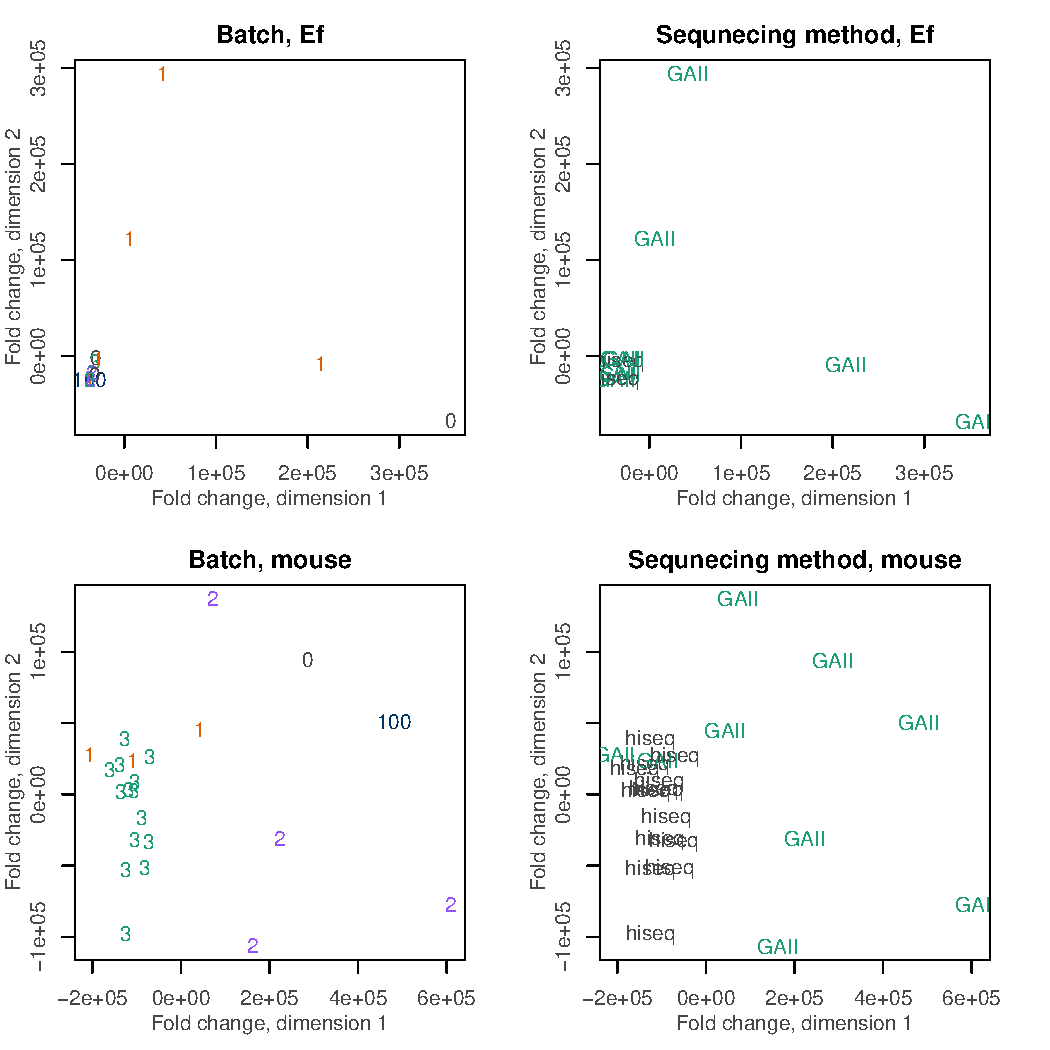
\includegraphics[width=\textwidth]{EfMm_4-mds.pdf} % Include 
	\caption{Multidimensional scaling shows no clear sample pattern due to technical variation. Effect on scaling is visualized for batch (left) and sequencing method (right). Upper panel displays \textit{E. falciformis} data and lower panel mouse data. Distances on plot approximate log2 fold changes. Scaling was done with Euclidean distance and "pairwise" gene selection method as implemented in R package limma (version 3.28.10).}
\end{center}
\end{figure}


%%%%%%%%%%%%%%%%%%%%%%%%%%%%%%%%%%%%%%%%%%%%%%%%%%%%%%%%%%%%%%%%%%%%%%%%%%
%% 	INPUT TO HEATMAP	
%%%%%%%%%%%%%%%%%%%%%%%%%%%%%%%%%%%%%%%%%%%%%%%%%%%%%%%%%%%%%%%%%%%%%%%%%%
\subsection{Differentially abundant mRNAs used for hierarchical clustering}

A selection of differently abundant mRNAs are used for hierarchical clustering of \textit{E. falciformis} life cycle relevant genes. In each comparison (see Table 3), the 500 differentially abundant mRNAs with lowest FDR are selected. In the next step, the 500 mRNAs from each comparison (or less) are joined (4935 genes) and only unique genes are selected (1618 genes). The 22 genes in the NMRI vs C57BL/6 comparison are not included in the \textit{E. falciformis} life cycle analysis.}

\setlength{\tabcolsep}{10pt}
\begin{table}[H]
%\begin{adjustwidth}{-10}{}
\small
\begin{center}
\caption{Differentially abundant mRNAs used for hierarchical clustering.}
\begin{tabular}{*2l}    \toprule
	\textit{Data description} & Number of genes \\ \midrule
	Sum of 1st infection NMRI sample differences	& 4935  \\ 
	(including oocysts and sporozoites)	\\	
	Used in hierarchical clustering (heatmap)  	& 1618 \\ 	\bottomrule	
\hline
\end{tabular}
\end{center}
%\end{adjustwidth}
\end{table}

%%%%%%%%%%%%%%%%%%%%%%%%%%%%%%%%%%%%%%%%%%%%%%%%%%%%%%%%%%%%%%%%%%%%%%%%%%
%% 	HEATMAPS
%%%%%%%%%%%%%%%%%%%%%%%%%%%%%%%%%%%%%%%%%%%%%%%%%%%%%%%%%%%%%%%%%%%%%%%%%%

\clearpage
\subsection{First versus second infection, mouse}
\begin{figure}[h!]
%\begin{center}
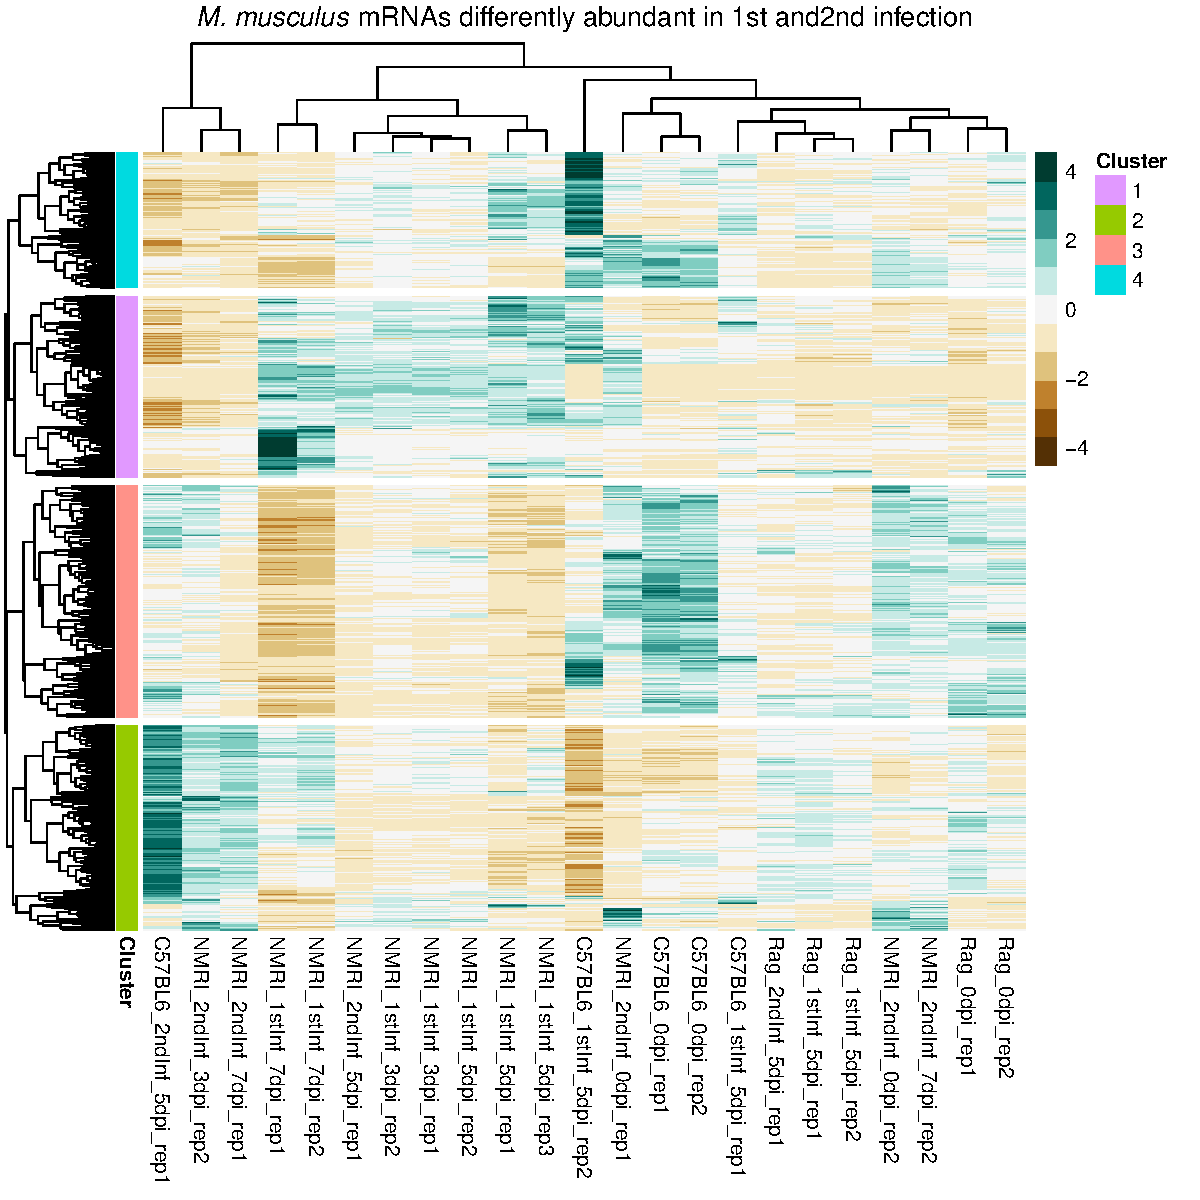
\includegraphics[width=\linewidth]{Mm1st2ndHeatmap.pdf}  
	\caption{Mouse mRNAs with significantly different abundance between first infection and challenge infection (see Table 2). Samples do not cluster into first and second infection clusters. The two major sample cluster each contain four challenge infection samples.}
%\end{center}
\end{figure}

\subsection{Differences between mouse strains,\textit{E. falciformis}}
\begin{figure}[H]
\begin{center}
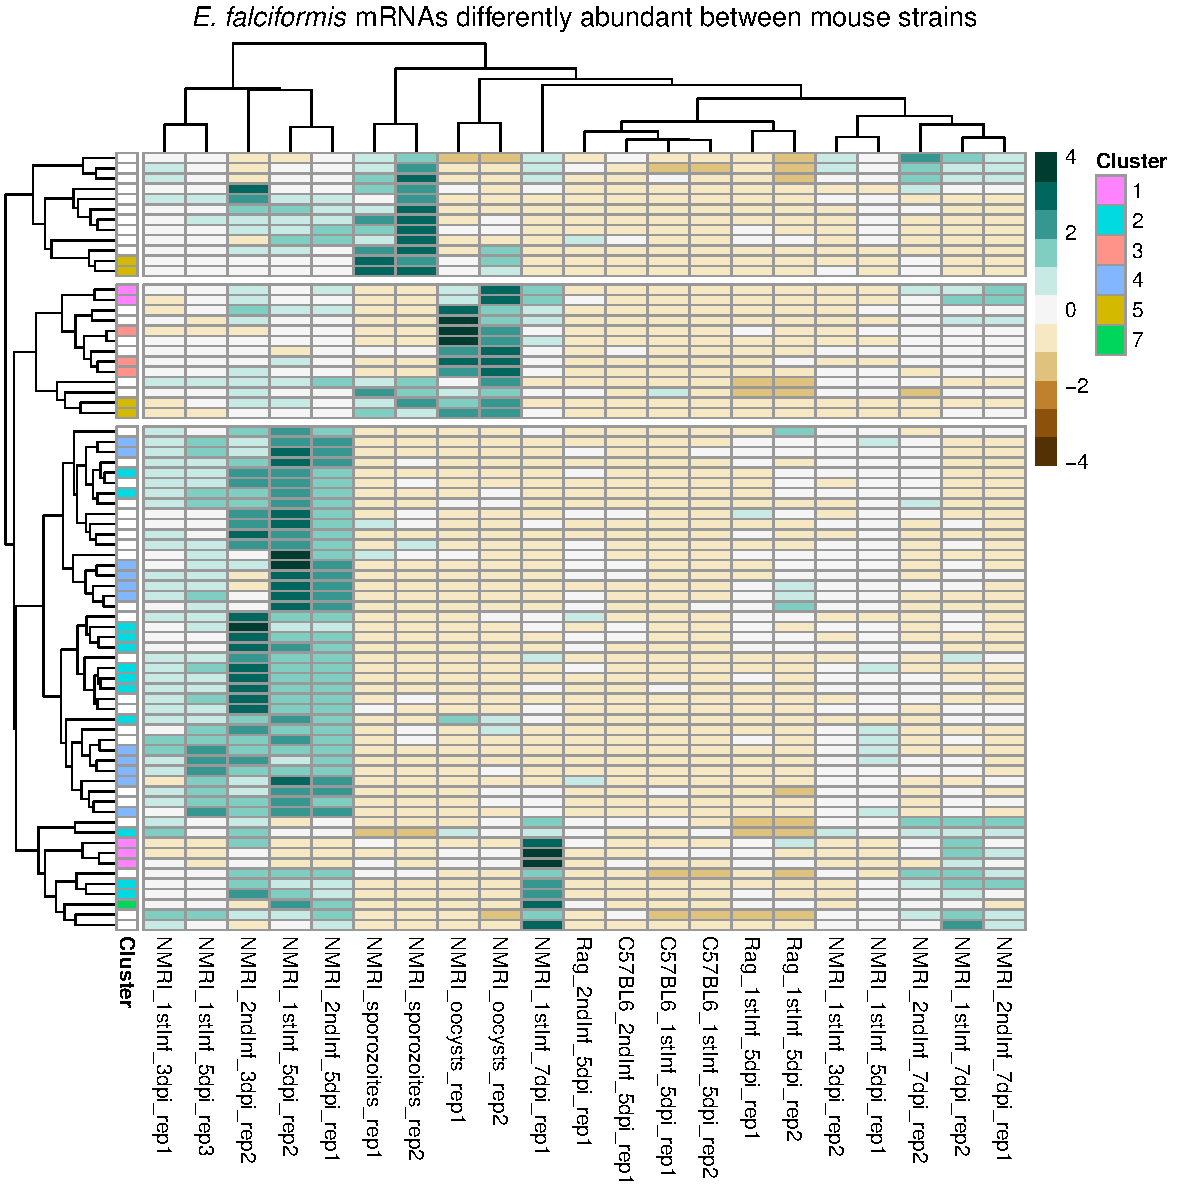
\includegraphics[width=\textwidth]{EfStrainHeatmap.pdf}  
	\caption{\textit{E. falciformis} with Euclidean distance .........as implemented in R package limma.}
\end{center}
\end{figure}

\subsection{Differences between mouse strains, mouse}
\begin{figure}[H]
\begin{center}
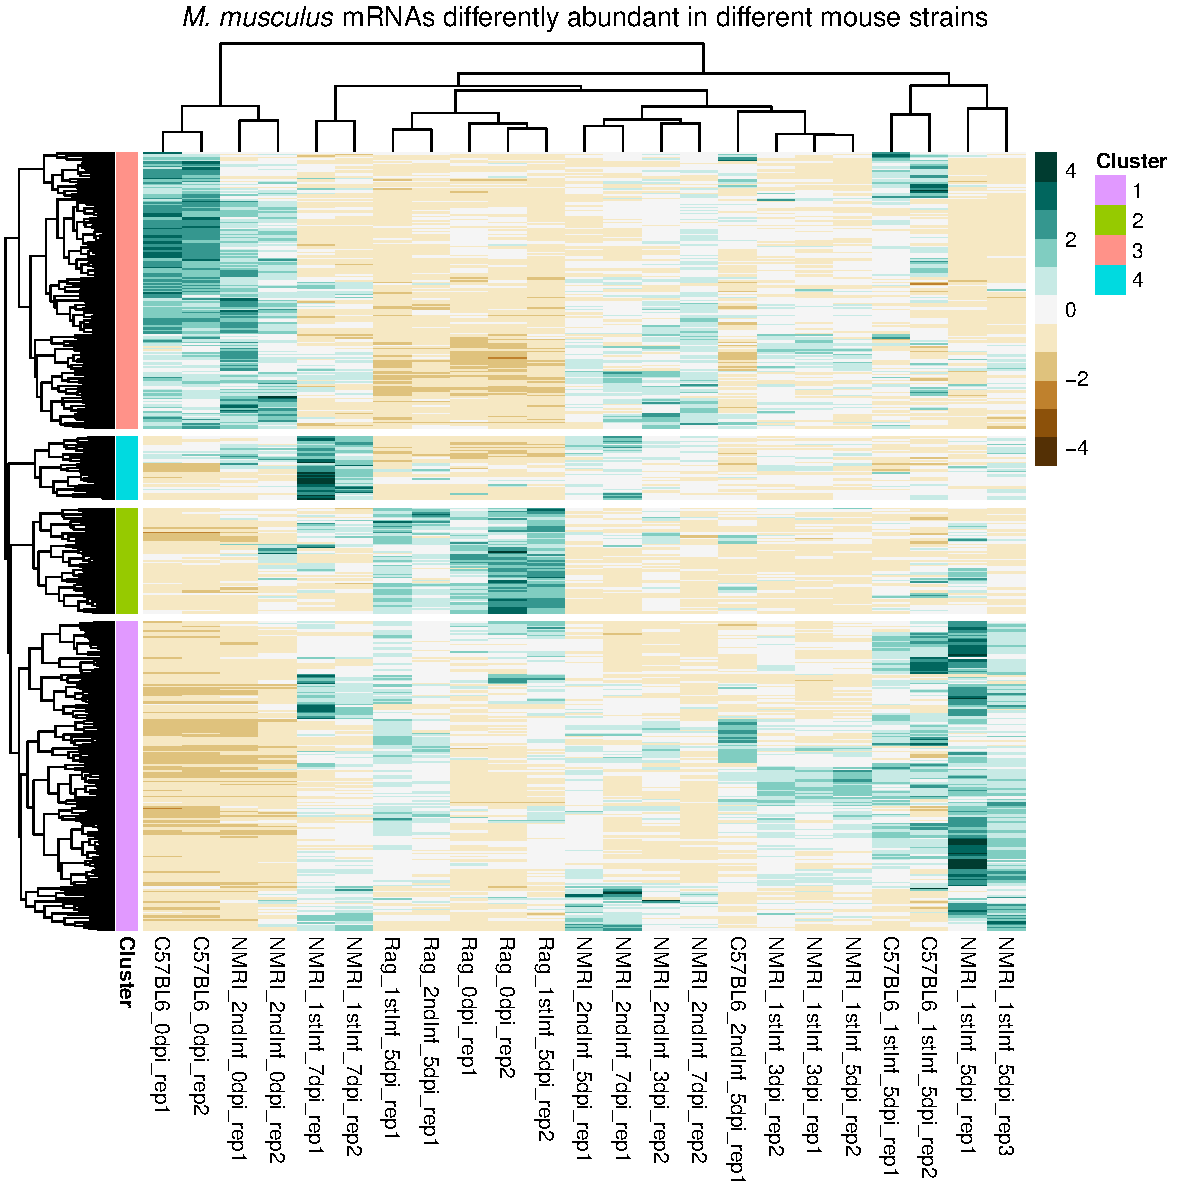
\includegraphics[width=\textwidth]{MmStrainHeatmap.pdf}  
	\caption{Mouse.... with Euclidean distance .........as implemented in R package limma.}
\end{center}
\end{figure}


\end{document}

